% Бүлэг 2

\chapter{Системийн шинжилгээ}
\label{Chapter2}

% Юзкейсийн тодорхойлолтын хүснэгт: {нэр}{ID}{үндсэн}{нэмэлт}{товч}{өмнөх}{урсгал}{дараах}{алтернатив}
\newcommand{\usecase}[9]{%
\begin{longtable}{|p{3.4cm}|p{11.2cm}|}
\caption{#1 юзкейсийн тодорхойлолт}\label{table:uc#2}\\ \hline
\textbf{Юзкейс:} & #1 \\ \hline
\textbf{ID:} & UC-#2 \\ \hline
\textbf{Үүсгэсэн:} & \shortname \\ \hline
\textbf{Үүсгэсэн огноо:} & 2026.09.29 \\ \hline
\textbf{Үндсэн тоглогч:} & #3 \\ \hline
\textbf{Нэмэлт тоглогч:} & #4 \\ \hline
\textbf{Товч тайлбар:} & #5 \\ \hline
\textbf{Өмнөх нөхцөл:} & #6 \\ \hline
\textbf{Үндсэн урсгал:} & #7 \\ \hline
\textbf{Дараах нөхцөл:} & #8 \\ \hline
\textbf{Алтернатив урсгал:} & #9 \\ \hline
\end{longtable}}

%-------------------------------------------------------------------------------
\section{Системийн үйл ажиллагаа}
Одоогийн байдлаар 5S, lean аргачлал хэрэглэдэг байгууллагуудад аудитын шалгах хуудас цаасаар бөглөгдөж, дараа нь хүснэгтэд шивэгдэнэ; ажлын даалгавар ам болон чатаар өгөгдөнө; сарын тайланг хэлтэс бүрийн мэдээллээс гараар нэгтгэнэ. Шинэ систем эдгээр урсгалыг нэг өгөгдлийн сан дээр нэгтгэж, мэдээллийг үүссэн газарт нь (цех дээр, гар утаснаас) бүртгэх боломж олгоно. Системийн үйл ажиллагааг хэрэглэгчийн дүрээр тайлбарлавал:

\paragraph{}\textbf{Ажилтан}: өөрт оноосон ажлыг ``хоцорсон, өнөөдөр, энэ долоо хоногт'' гэсэн дарааллаар харж, нэг товшилтоор дуусгана. Өдрийн бүртгэл, долоо хоногийн тайлан бичнэ. Талбайн QR шошгыг гар утсаар уншуулж 5S аудит хийж, улаан шошго, дутагдлыг зурагтай бүртгэнэ. Сайжруулалтын санаа илгээж, хариуг нь мэдэгдлээр авна. Сүлжээгүй үед хийсэн бүртгэл утсанд хадгалагдана.

\paragraph{}\textbf{Менежер}: ажилтны бүх үйлдлийг хийхээс гадна төсөл, ажил үүсгэж хариуцагч, хугацаа онооно. Явцын самбар, өглөөний хурлын самбараас хоцорсон, хариуцагчгүй ажлыг харна. Gemba явалт бүртгэж, санааг хянана. Сарын тайлангийн тойм бичвэрийг бичиж батална.

\paragraph{}\textbf{Админ}: менежерийн бүх үйлдлийг хийхээс гадна хэрэглэгч урьж, эрх олгоно; хэлтэс, 5S талбай, аудитын загвар, байгууллагын тохиргоог удирдана.

\paragraph{}\textbf{Систем (цагийн хуваарь)}: өглөө бүр дуусах, хоцорсон ажлын сануулга илгээнэ; талбайн аудитын давтамжийн дагуу аудитын ажил үүсгэнэ; сар дуусахад тайланг хааж архивлана.

%-------------------------------------------------------------------------------
\section{Системийг ашиглах хэрэглэгчид}
Хэрэглэгчийн дүрүүд үүрлэсэн (ажиглагч $\subset$ ажилтан $\subset$ менежер $\subset$ админ) бөгөөд дээд дүр доод дүрийн бүх эрхийг өвлөнө (Хүснэгт~\ref{table:roles}).

\begin{table}[H]
\centering
\caption{Хэрэглэгчийн дүр ба эрх}
\label{table:roles}
\begin{tabular}{|p{2.8cm}|p{4.4cm}|p{7.2cm}|}
\hline
\textbf{Дүр} & \textbf{Тайлбар} & \textbf{Гол эрхүүд} \\ \hline
Ажиглагч & Удирдлага, зөвлөх зэрэг зөвхөн хардаг хэрэглэгч & Ажил, аудит, тайлан, санаа унших; мэдэгдэл унших \\ \hline
Ажилтан & Цех, оффисын ажилтан & Өөрт оноосон ажил шинэчлэх, өдрийн бүртгэл, аудит, улаан шошго, санаа, долоо хоногийн тайлан \\ \hline
Менежер & Хэлтэс, багийн удирдлага & Ажил, төсөл үүсгэх, оноох; сарын тайлан хаах; санаа хянах; Gemba явалт; хэрэглэгч урих \\ \hline
Админ & Байгууллагын систем хариуцагч & Хэрэглэгч, хэлтэс, талбай, загвар, тохиргоо; өөрөөсөө доод түвшний эрх олгох \\ \hline
\end{tabular}
\end{table}

%-------------------------------------------------------------------------------
\section{Функциональ шаардлага}
Функциональ шаардлагыг MoSCoW аргаар эрэмбэлэв (M -- заавал, S -- байх ёстой, C -- байж болно).

\begin{longtable}{|p{1.4cm}|p{9.6cm}|p{2.4cm}|c|}
\caption{Функциональ шаардлага}\label{table:fr}\\ \hline
\textbf{Код} & \textbf{Шаардлага} & \textbf{Дүр} & \textbf{Эр.} \\ \hline
\endfirsthead
\hline
\textbf{Код} & \textbf{Шаардлага} & \textbf{Дүр} & \textbf{Эр.} \\ \hline
\endhead
FR-01 & Хэрэглэгч и-мэйл, нууц үгээр нэвтэрч, эрхийнхээ хүрээнд системийг ашиглана & Бүгд & M \\ \hline
FR-02 & Админ хэрэглэгчийг урилгаар нэмж, өөрөөсөө доод түвшний эрх олгоно & Админ & M \\ \hline
FR-03 & Менежер ажил үүсгэж, хариуцагч, хугацаа, ач холбогдол онооно & Менежер & M \\ \hline
FR-04 & Ажилтан өөрт оноосон ажлыг хоцорсон, өнөөдөр, энэ долоо хоног гэж эрэмбэлж харна & Ажилтан & M \\ \hline
FR-05 & Ажил оноогдоход болон өглөө бүр дуусах, хоцорсон ажлын талаар мэдэгдэл ирнэ & Ажилтан & M \\ \hline
FR-06 & Менежер 5S талбайн зураг зурж, бүс бүрт хариуцагч, стандарт зураг, аудитын давтамж онооно & Менежер & M \\ \hline
FR-07 & Ажилтан бүсийн QR шошгыг уншуулж, шалгах хуудсаар аудит хийнэ & Ажилтан & M \\ \hline
FR-08 & Аудитын оноо босгоос доош бол бүсийн хариуцагчид засах ажил автоматаар үүснэ & Систем & M \\ \hline
FR-09 & Ажилтан улаан шошго болон дутагдлыг зурагтай бүртгэнэ & Ажилтан & M \\ \hline
FR-10 & Ажилтан өдрийн бүртгэл (юу хийсэн, дараа нь юу хийх) хөтөлнө & Ажилтан & M \\ \hline
FR-11 & Ажилтан долоо хоногийн тайлан бичнэ; пүрэв, баасан гарагт сануулга гарна & Ажилтан & S \\ \hline
FR-12 & Сарын тайлан бүртгэлээс автоматаар бүрдэж, тогтсон өдөр хаагдан архивлагдана & Систем & M \\ \hline
FR-13 & Хагас жилийн, жилийн тайлан хаагдсан сарын тайлангаас нэгтгэгдэнэ & Менежер & S \\ \hline
FR-14 & Менежер сарын тайлангийн тойм бичвэрийг AI-аар ноороглуулж, засаад батална & Менежер & C \\ \hline
FR-15 & Өглөөний хурлын самбар өчигдөр, өнөөдөр, анхаарах зүйл, 5S, Gemba-г харуулна & Менежер & S \\ \hline
FR-16 & Менежер Gemba явалт бүртгэж, дараагийн алхам бүр ажил болно & Менежер & S \\ \hline
FR-17 & Ажилтан сайжруулалтын санаа илгээж, менежер хянаж хариу өгнө & Ажилтан, менежер & S \\ \hline
FR-18 & Гар утасны апп сүлжээгүй үед хийсэн өөрчлөлтийг хадгалж, дараа илгээнэ & Ажилтан & M \\ \hline
FR-19 & Систем монгол, англи хэлээр ажиллана & Бүгд & M \\ \hline
FR-20 & Байгууллагын үйл ажиллагааны түүх (аудитын бүртгэл, архив) хадгалагдана & Админ & S \\ \hline
FR-21 & Хэрэглэгч бүртгэлээ устгах хүсэлт гаргана & Бүгд & S \\ \hline
FR-22 & Удирдлага туршилтын үзүүлэлтүүдийг (K1--K6, \ref{sec:kpi}-р хэсэг) сар, долоо хоногоор харна & Менежер & S \\ \hline
\end{longtable}

%-------------------------------------------------------------------------------
\section{Функциональ бус шаардлага}
\begin{longtable}{|p{1.6cm}|p{3.2cm}|p{9.6cm}|}
\caption{Функциональ бус шаардлага (ISO/IEC 25010)}\label{table:nfr}\\ \hline
\textbf{Код} & \textbf{Шинж} & \textbf{Шаардлага} \\ \hline
\endfirsthead
\hline
\textbf{Код} & \textbf{Шинж} & \textbf{Шаардлага} \\ \hline
\endhead
NFR-01 & Аюулгүй байдал & Нууц үг hash-лагдаж хадгалагдана; бүх хүсэлт JWT-ээр баталгаажна; эрхийг сервер тал дээр шалгана \\ \hline
NFR-02 & Аюулгүй байдал & Байгууллага бүрийн өгөгдөл тусгаарлагдана; нэг байгууллага нөгөөгийнхийг харахгүй \\ \hline
NFR-03 & Хэрэглэхэд хялбар & WCAG 2.1 AA хүртээмж~\cite{wcag}; SUS оноо 68-аас дээш~\cite{brooke} \\ \hline
NFR-04 & Хэрэглэхэд хялбар & Гар утсанд нэг гараар ашиглах, том үсэг, бараан горимд зохицно \\ \hline
NFR-05 & Найдвартай байдал & Сүлжээ тасрахад өгөгдөл алдагдахгүй; давхар илгээлтээс сэргийлнэ \\ \hline
NFR-06 & Гүйцэтгэл & Гол хуудас энгийн сүлжээнд 2 секундээс бага хугацаанд ачаална \\ \hline
NFR-07 & Засварлагдах чанар & Өгөгдлийн сангийн өөрчлөлт migration-оор; автомат тестийн хамрах хүрээ \\ \hline
NFR-08 & Зөөвөрлөх чанар & Docker-оор аль ч Linux сервер дээр байршина \\ \hline
NFR-09 & Нууцлал & AI үйлчилгээ рүү зөвхөн нэргүй, нэгдсэн тоо баримт илгээгдэнэ \\ \hline
NFR-10 & Цаг хугацаа & Огноо, сануулга байгууллагын цагийн бүсээр (Asia/Ulaanbaatar) тооцогдоно \\ \hline
\end{longtable}

%-------------------------------------------------------------------------------
\section{Use Case диаграмм}
Зураг~\ref{fig:usecase}-т системийн оролцогчид болон тэдгээрийн гүйцэтгэх гол use-case-уудыг харуулав. Менежер ажилтны, админ менежерийн бүх use-case-ийг өвлөнө.

\begin{figure}[H]
\centering
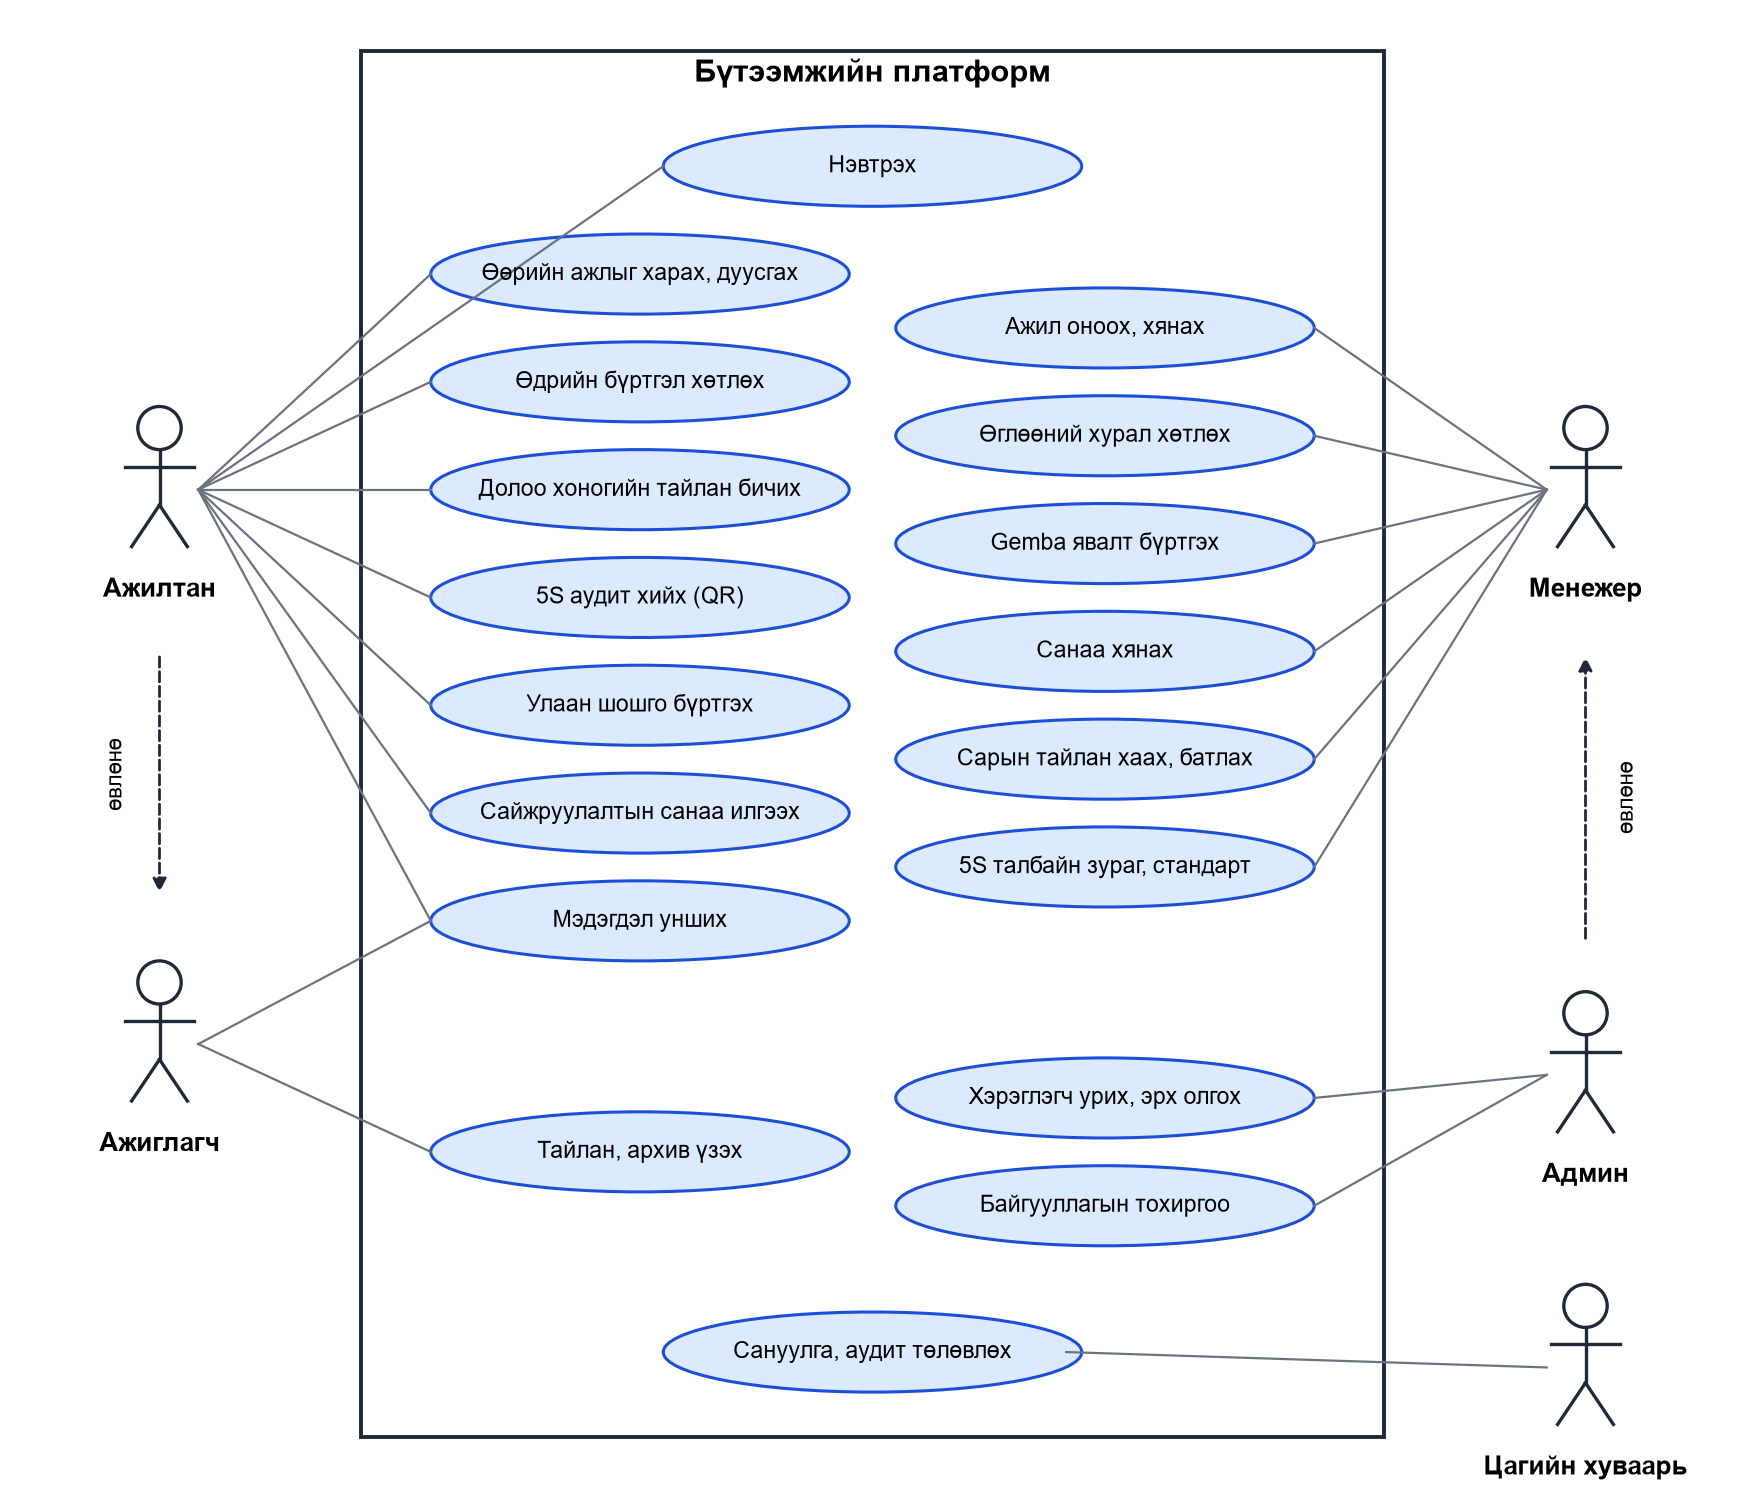
\includegraphics[width=\linewidth]{Figures/usecase.png}
\caption{Юзкейс диаграмм}
\label{fig:usecase}
\end{figure}

%-------------------------------------------------------------------------------
\section{Юзкейс диаграммын тодорхойлолт}
Гол use-case-уудын тодорхойлолтыг Хүснэгт~\ref{table:uc01}--\ref{table:uc09}-д харуулав~\cite{cockburn}.

\usecase{Нэвтрэх}{01}{Хэрэглэгч}{Байхгүй}
{Бүртгэлтэй хэрэглэгч системд нэвтэрнэ.}
{Хэрэглэгч идэвхтэй бүртгэлтэй байх.}
{1. Хэрэглэгч и-мэйл, нууц үгээ оруулж ``Нэвтрэх'' дарна.\par
 2. Систем и-мэйлээр хэрэглэгчийг хайж, нууц үгийн hash-ийг шалгана.\par
 3. Систем access, refresh токен үүсгэнэ.\par
 4. Систем хэрэглэгчийн эрхэд тохирсон нүүр хуудсыг харуулна.}
{Хэрэглэгч нэвтэрсэн, токен хадгалагдсан байна.}
{2а. Нууц үг буруу эсвэл бүртгэл идэвхгүй бол алдааны мэдэгдэл харуулна.}

\usecase{5S аудит хийх}{02}{Ажилтан}{Систем}
{Бүсийн 5S түвшинг шалгах хуудсаар хэмжиж, дутагдлыг бүртгэнэ.}
{Хэрэглэгч нэвтэрсэн; бүс нь аудитын загвартай; audits:create эрхтэй.}
{1. Ажилтан бүсийн QR шошгыг уншуулна.\par
 2. Систем бүсийн шалгах хуудас, стандарт зургийг харуулна.\par
 3. Ажилтан асуулт бүрт оноо эсвэл тийм/үгүй хариулт өгч, шаардлагатай бол зураг хавсаргана.\par
 4. Ажилтан ``Дуусгах'' дарна.\par
 5. Систем оноог тооцоолж хадгалж, бүсийн сүүлийн оноог шинэчилнэ.\par
 6. Оноо 85\%-иас доош бол систем бүсийн хариуцагчид засах ажил үүсгэж мэдэгдэнэ.}
{Аудитын бүртгэл, бүсийн оноо, шаардлагатай бол засах ажил үүссэн байна.}
{5а. Сүлжээгүй бол аудит утсанд хадгалагдаж, сүлжээ сэргэхэд илгээгдэнэ.\par
 6а. Тухайн аудитаас ажил үүссэн бол давхар үүсгэхгүй.}

\usecase{Ажил оноох}{03}{Менежер}{Ажилтан}
{Ажлыг хариуцагчтай, хугацаатай оноож, биелэлтийг хянана.}
{Менежер tasks:create эрхтэй; хариуцагч идэвхтэй хэрэглэгч.}
{1. Менежер ажлын нэр, тайлбар, хариуцагч, хугацаа, ач холбогдлыг оруулна.\par
 2. Систем эрхийг шалгаж, ажлыг хадгална.\par
 3. Систем хариуцагчид мэдэгдэл илгээнэ.\par
 4. Ажилтан ажлын төлвийг ``хийгдэж байна'', ``дууссан'' болгоно.\par
 5. Менежер явцын самбараас биелэлтийг харна.}
{Ажил хариуцагчтай, хугацаатай бүртгэгдсэн байна.}
{2а. Эрхгүй бол 403 алдаа буцаана.\par
 4а. Хугацаа хэтэрвэл ажил ``хоцорсон'' бүлэгт орж өглөөний сануулгад багтана.}

\usecase{Сарын тайлан хаах}{04}{Систем (цагийн хуваарь)}{Менежер}
{Сарын үр дүнг автоматаар нэгтгэж, өөрчлөгдөхгүй хувилбараар архивлана.}
{Байгууллагын тохиргоонд сар хаах өдөр тодорхойлогдсон.}
{1. Систем цаг тутам байгууллага бүрийн цагийн бүсээр хаах өдөр болсон эсэхийг шалгана.\par
 2. Өнгөрсөн сар хаагдаагүй бол тухайн сарын бүртгэлүүдийг хуулбарлан хадгална.\par
 3. Менежер тайланг нээж, тойм бичвэр бичих эсвэл AI-аар ноороглуулна.\par
 4. Менежер бичвэрийг засаад батална.}
{Хаагдсан, архивлагдсан сарын тайлан бий болно.}
{1а. Сервер тухайн өглөө ажиллаагүй бол дараагийн ажиллалтаар хаана.\par
 3а. AI тохируулаагүй бол менежер гараар бичнэ.}

\usecase{Gemba явалт бүртгэх}{05}{Менежер}{Систем}
{Цех дээр ажигласан зүйл, ярилцлагыг бүртгэж, дараагийн алхмыг ажил болгоно.}
{Хэрэглэгч gemba:walk эрхтэй.}
{1. Менежер бүс эсвэл газрыг сонгоно.\par
 2. Ажигласан зүйл, хийсэн ярилцлагаа бичнэ.\par
 3. Дараагийн алхам бүрт нэр, хариуцагч оруулна.\par
 4. Систем явалтыг хадгалж, алхам бүрээс ажил үүсгэнэ.}
{Gemba явалтын бүртгэл ба хариуцагчтай ажлууд үүснэ.}
{3а. Хариуцагч сонгоогүй бол ажил явалт хийсэн менежерт оноогдоно.}

\usecase{Сайжруулалтын санаа илгээх}{06}{Ажилтан}{Менежер}
{Ажилтны санааг бүртгэж, шийдвэрийг санал гаргагчид мэдэгдэнэ.}
{Ажилтан ideas:create, менежер ideas:review эрхтэй.}
{1. Ажилтан санааны гарчиг, тайлбар, зураг оруулж илгээнэ.\par
 2. Менежер санааг хянаж шийдвэр, хариу бичнэ.\par
 3. Систем санал гаргагчид мэдэгдэл илгээнэ.\par
 4. Батлагдсан санаанаас ажил үүснэ.}
{Санаа хариутай болж, шаардлагатай бол ажил үүснэ.}
{2а. Хянагдаагүй санаа өглөөний хурлын самбарт харагдана.}

\usecase{Долоо хоногийн тайлан бичих}{07}{Ажилтан}{Менежер}
{Долоо хоногийн үр дүн, төлөвлөгөө, саадыг товч бүртгэнэ.}
{Хэрэглэгч checkins:write эрхтэй.}
{1. Пүрэв, баасан гарагт тайлан бичээгүй ажилтанд сануулга гарна.\par
 2. Ажилтан хийсэн ажил, дараагийн төлөвлөгөө, саад бэрхшээлээ бичнэ.\par
 3. Систем хадгална.\par
 4. Менежер багийн тайлангуудыг нэг дор уншина.}
{Долоо хоногийн тайлан хадгалагдана.}
{2а. Сүлжээгүй бол утсанд хадгалагдана.}

\usecase{Өглөөний хурал хөтлөх}{08}{Менежер}{Ажилтан}
{Ээлжийн эхэнд багийн өчигдрийн үр дүн, өнөөдрийн ажил, анхаарах асуудлыг нэг дэлгэцээс хэлэлцэнэ.}
{Менежер нэвтэрсэн; хэлтэст ажилтнууд бүртгэлтэй.}
{1. Менежер ``Өглөөний хурал'' хуудсыг нээж, хэлтсээ сонгоно.\par
 2. Систем өчигдөр дууссан ажил, аудитын дундаж, өнөөдөр дуусах ажил, хоцорсон ба хариуцагчгүй ажил, стандартаас доош 5S бүс, хянагдаагүй санаа, Gemba-гийн биелэлтийг харуулна.\par
 3. Менежер хоцорсон ажлын хариуцагч, хугацааг хэлэлцэж шийдвэрлэнэ.\par
 4. Систем тоо баримтыг хоёр минут тутамд шинэчилнэ.}
{Баг өдрийн тэргүүлэх ажил, шийдвэр шаардсан асуудлаа тохирсон байна.}
{1а. Том дэлгэцэд бүтэн дэлгэцийн горимоор харуулна.}

\usecase{5S талбай, стандарт тохируулах}{09}{Админ, менежер}{Ажилтан}
{Байгууллагын талбайн зургийг зурж, бүс бүрт хариуцагч, стандарт зураг, аудитын давтамж онооно.}
{Хэрэглэгч zones:update эрхтэй.}
{1. Менежер талбайн зураг (давхар, бүс, объект)-ыг зурах эсвэл зураг оруулна.\par
 2. Бүс бүрт нэр, код, хариуцагч, стандарт зураг, аудитын шат, давтамжийг онооно.\par
 3. Систем өөрчлөлтийг хувилбараар хадгалж, бүс бүрийн QR шошгыг үүсгэнэ.\par
 4. Цагийн хуваарь давтамжийн дагуу аудитын ажил үүсгэнэ.}
{Бүсүүд хариуцагчтай, стандарттай, аудитын хуваарьтай болно.}
{3а. Өмнөх хувилбарыг сэргээх боломжтой.}

%-------------------------------------------------------------------------------
\section{Шаардлагын мөрдөх матриц}
Шаардлага бүр аль use-case-ээр хэрэгжиж, одоогийн байдлаар хаана хүрснийг Хүснэгт~\ref{table:trace}-д харуулав. Хэрэгжилтийг гурван түвшинд ялгав: \textbf{Код} -- системд хэрэгжсэн, \textbf{Тест} -- автомат тестээр баталгаажсан, \textbf{Туршилт} -- бодит байгууллагад ашиглаж хэмжсэн (\yes~бүрэн, $\sim$~хэсэгчлэн, --~хараахан үгүй).

\begin{longtable}{|p{1.3cm}|p{6.2cm}|p{1.6cm}|c|c|c|}
\caption{Шаардлагын мөрдөх матриц ба хэрэгжилтийн төлөв}\label{table:trace}\\ \hline
\textbf{Код} & \textbf{Шаардлага} & \textbf{Use-case} & \textbf{Код} & \textbf{Тест} & \textbf{Туршилт} \\ \hline
\endfirsthead
\hline
\textbf{Код} & \textbf{Шаардлага} & \textbf{Use-case} & \textbf{Код} & \textbf{Тест} & \textbf{Туршилт} \\ \hline
\endhead
FR-01 & Нэвтрэх, эрхийн хүрээ & UC-01 & \yes & \yes & -- \\ \hline
FR-02 & Урилга, эрх олгох & -- & \yes & \yes & -- \\ \hline
FR-03 & Ажил үүсгэх, оноох & UC-03 & \yes & \yes & -- \\ \hline
FR-04 & Ажлыг ач холбогдлоор харах & UC-03 & \yes & \yes & -- \\ \hline
FR-05 & Оноолт ба өглөөний мэдэгдэл & UC-03 & \yes & \yes & -- \\ \hline
FR-06 & 5S талбай, бүс, стандарт & UC-09 & \yes & \yes & -- \\ \hline
FR-07 & QR-ээр аудит хийх & UC-02 & \yes & \yes & -- \\ \hline
FR-08 & Аудитаас засах ажил & UC-02 & \yes & \yes & -- \\ \hline
FR-09 & Улаан шошго, зураг & UC-02 & \yes & \yes & -- \\ \hline
FR-10 & Өдрийн бүртгэл & UC-07 & \yes & \yes & -- \\ \hline
FR-11 & Долоо хоногийн тайлан, сануулга & UC-07 & \yes & \yes & -- \\ \hline
FR-12 & Сарын тайлан, хаалт, архив & UC-04 & \yes & \yes & -- \\ \hline
FR-13 & Хагас жил, жилийн тайлан & UC-04 & \yes & \yes & -- \\ \hline
FR-14 & AI тойм бичвэр & UC-04 & \yes & $\sim$ & -- \\ \hline
FR-15 & Өглөөний хурлын самбар & UC-08 & \yes & \yes & -- \\ \hline
FR-16 & Gemba явалт & UC-05 & \yes & \yes & -- \\ \hline
FR-17 & Сайжруулалтын санаа & UC-06 & \yes & \yes & -- \\ \hline
FR-18 & Сүлжээгүй горим & UC-02, 05, 07 & $\sim$ & \yes & -- \\ \hline
FR-19 & Монгол, англи хэл & бүгд & \yes & \yes & -- \\ \hline
FR-20 & Үйл ажиллагааны түүх, архив & UC-04 & \yes & \yes & -- \\ \hline
FR-21 & Бүртгэл устгах хүсэлт & -- & \yes & \yes & -- \\ \hline
FR-22 & KPI самбар (K1--K6) & UC-04, 08 & $\sim$ & -- & -- \\ \hline
\end{longtable}

FR-14-ийн AI дуудлагыг хиймэл хариугаар тестэлсэн бөгөөд бодит түлхүүрээр туршаагүй. FR-18-ийн сүлжээгүй горим нь бичих үйлдлүүдэд хэрэгжсэн, өгөгдлийг бүрэн офлайнаар унших нь хамрах хүрээнд ороогүй. Бүх шаардлагын ``Туршилт'' баганыг гуравдугаар үзлэгийн туршилтын ажиллагаагаар бөглөнө.

%-------------------------------------------------------------------------------
\section{Шинжилгээний класс диаграмм}
Зураг~\ref{fig:classA}-д системийн домэйн классууд, тэдгээрийн шинж чанар, хамаарлыг харуулав. Ажил (Task) нь аудит, Gemba явалт, санаанаас үүсэх бөгөөд sourceType, sourceId талбараар эх сурвалжаа хадгална.

\begin{figure}[H]
\centering
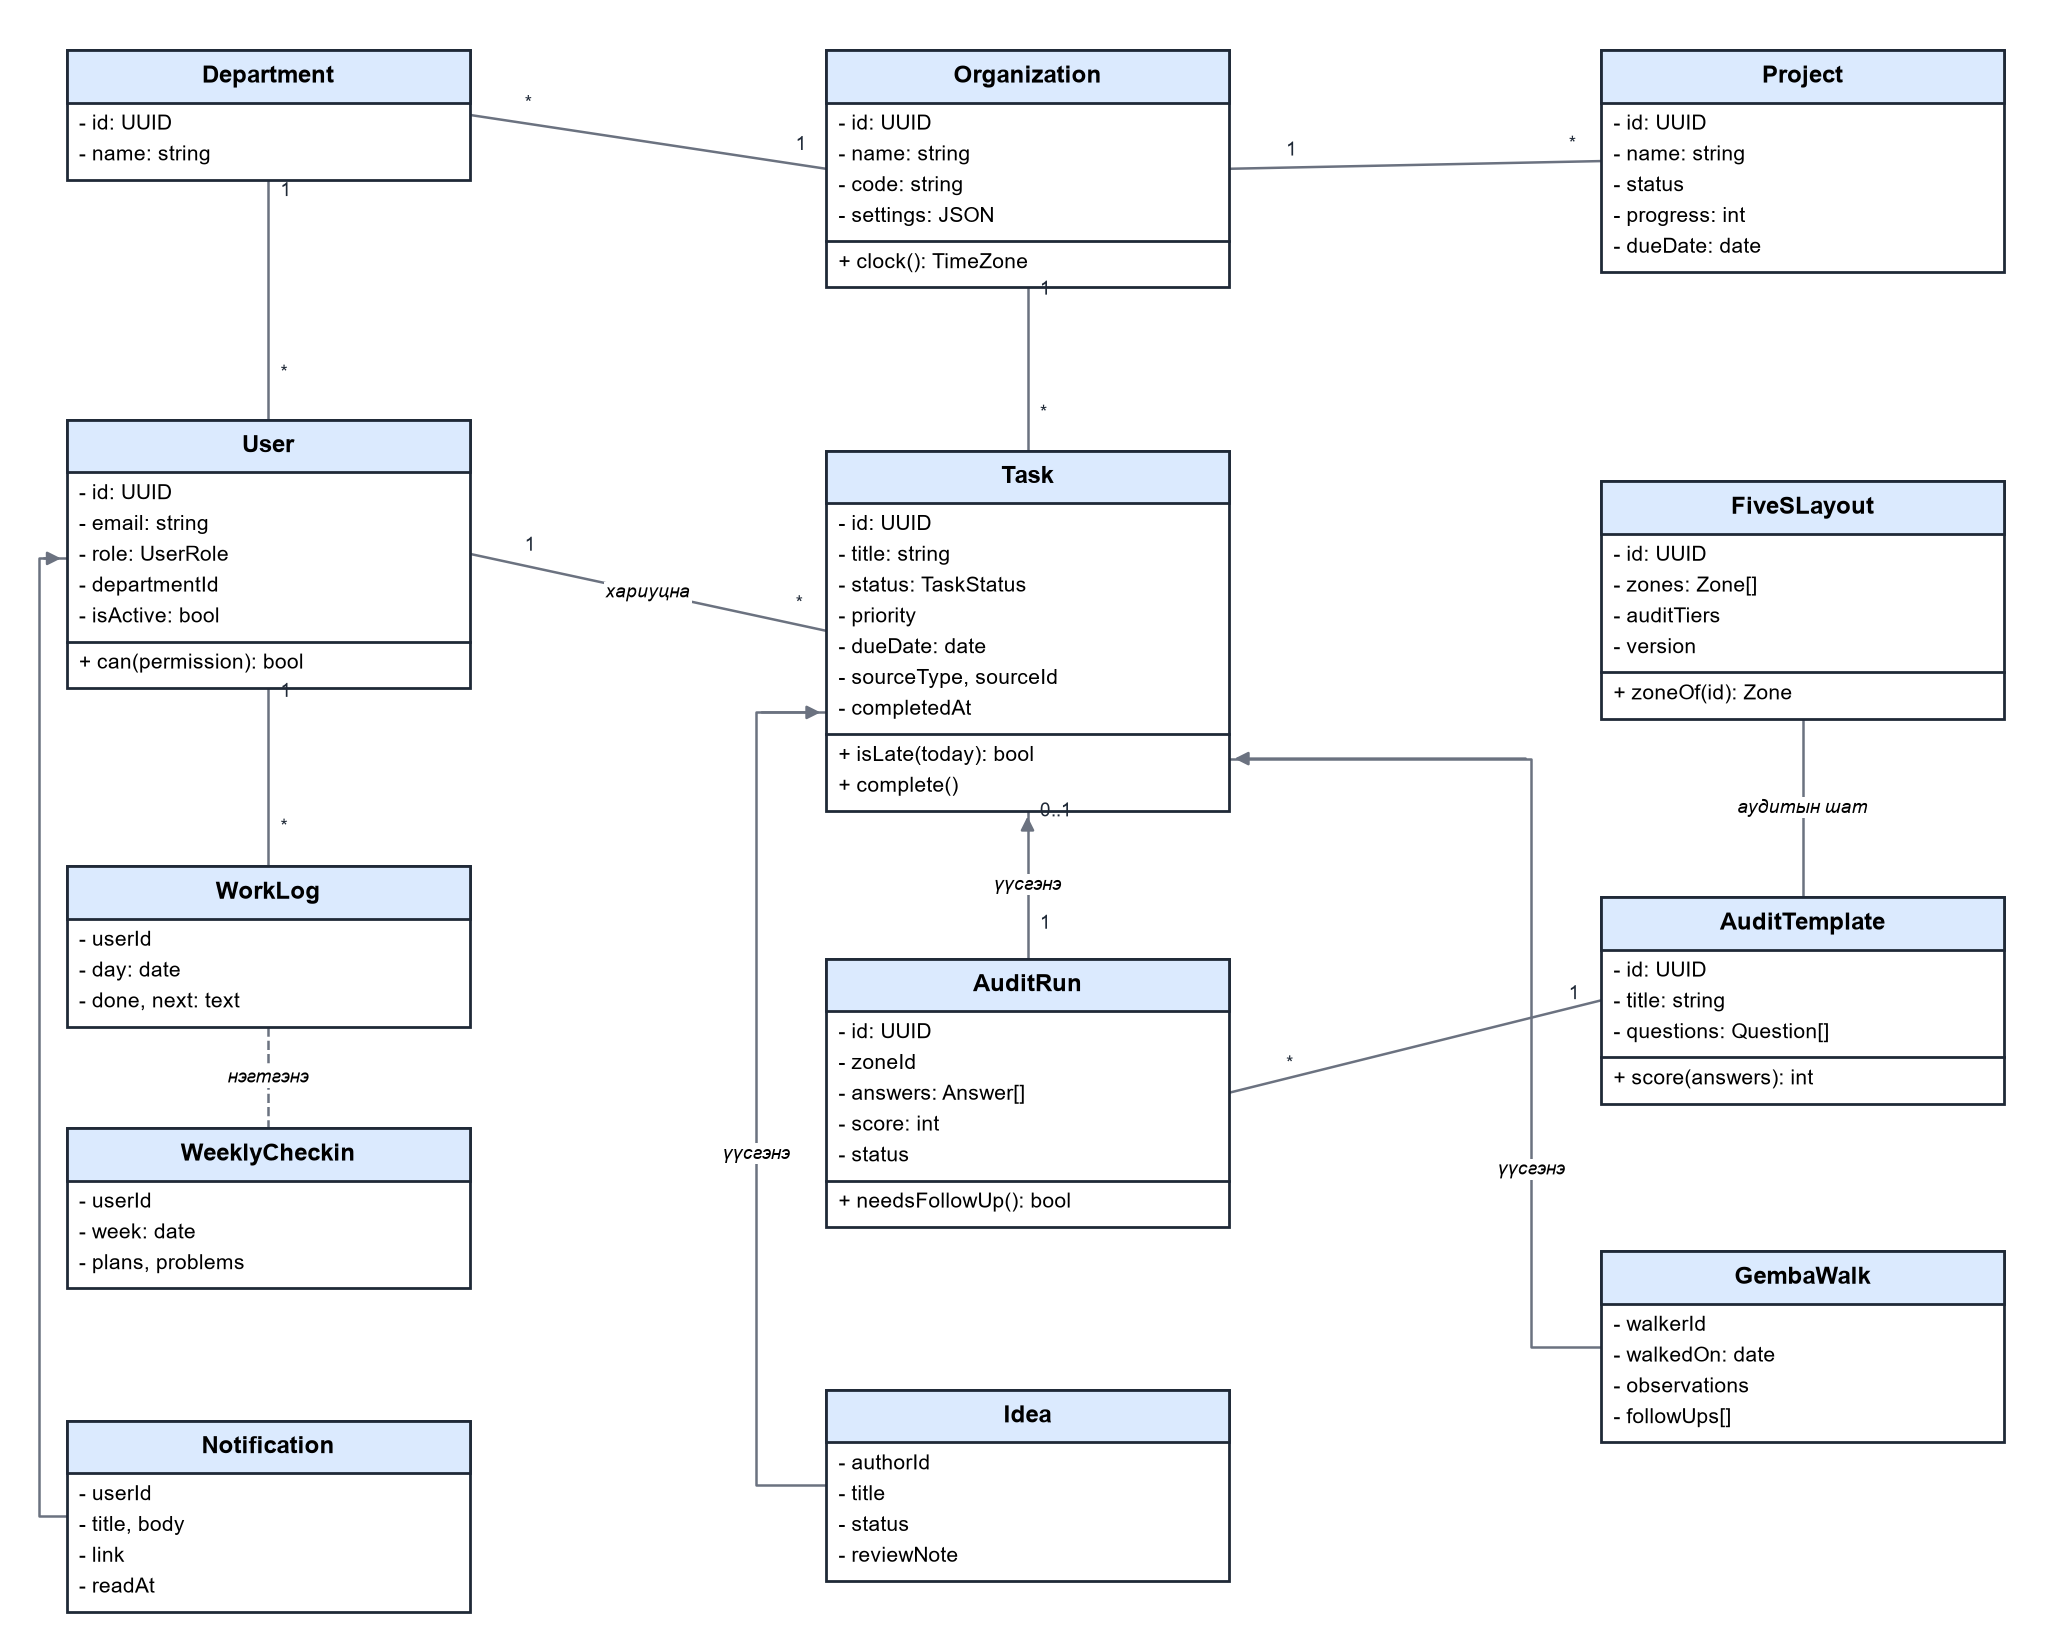
\includegraphics[width=\linewidth]{Figures/class_analysis.png}
\caption{Шинжилгээний класс диаграмм}
\label{fig:classA}
\end{figure}

%-------------------------------------------------------------------------------
\section{Шинжилгээний дарааллын диаграмм}
Зураг~\ref{fig:seqLogin}-д нэвтрэх, Зураг~\ref{fig:seqTask}-д ажил оноох үйл явцын объектуудын хоорондох мессежийн дарааллыг харуулав.

\begin{figure}[H]
\centering
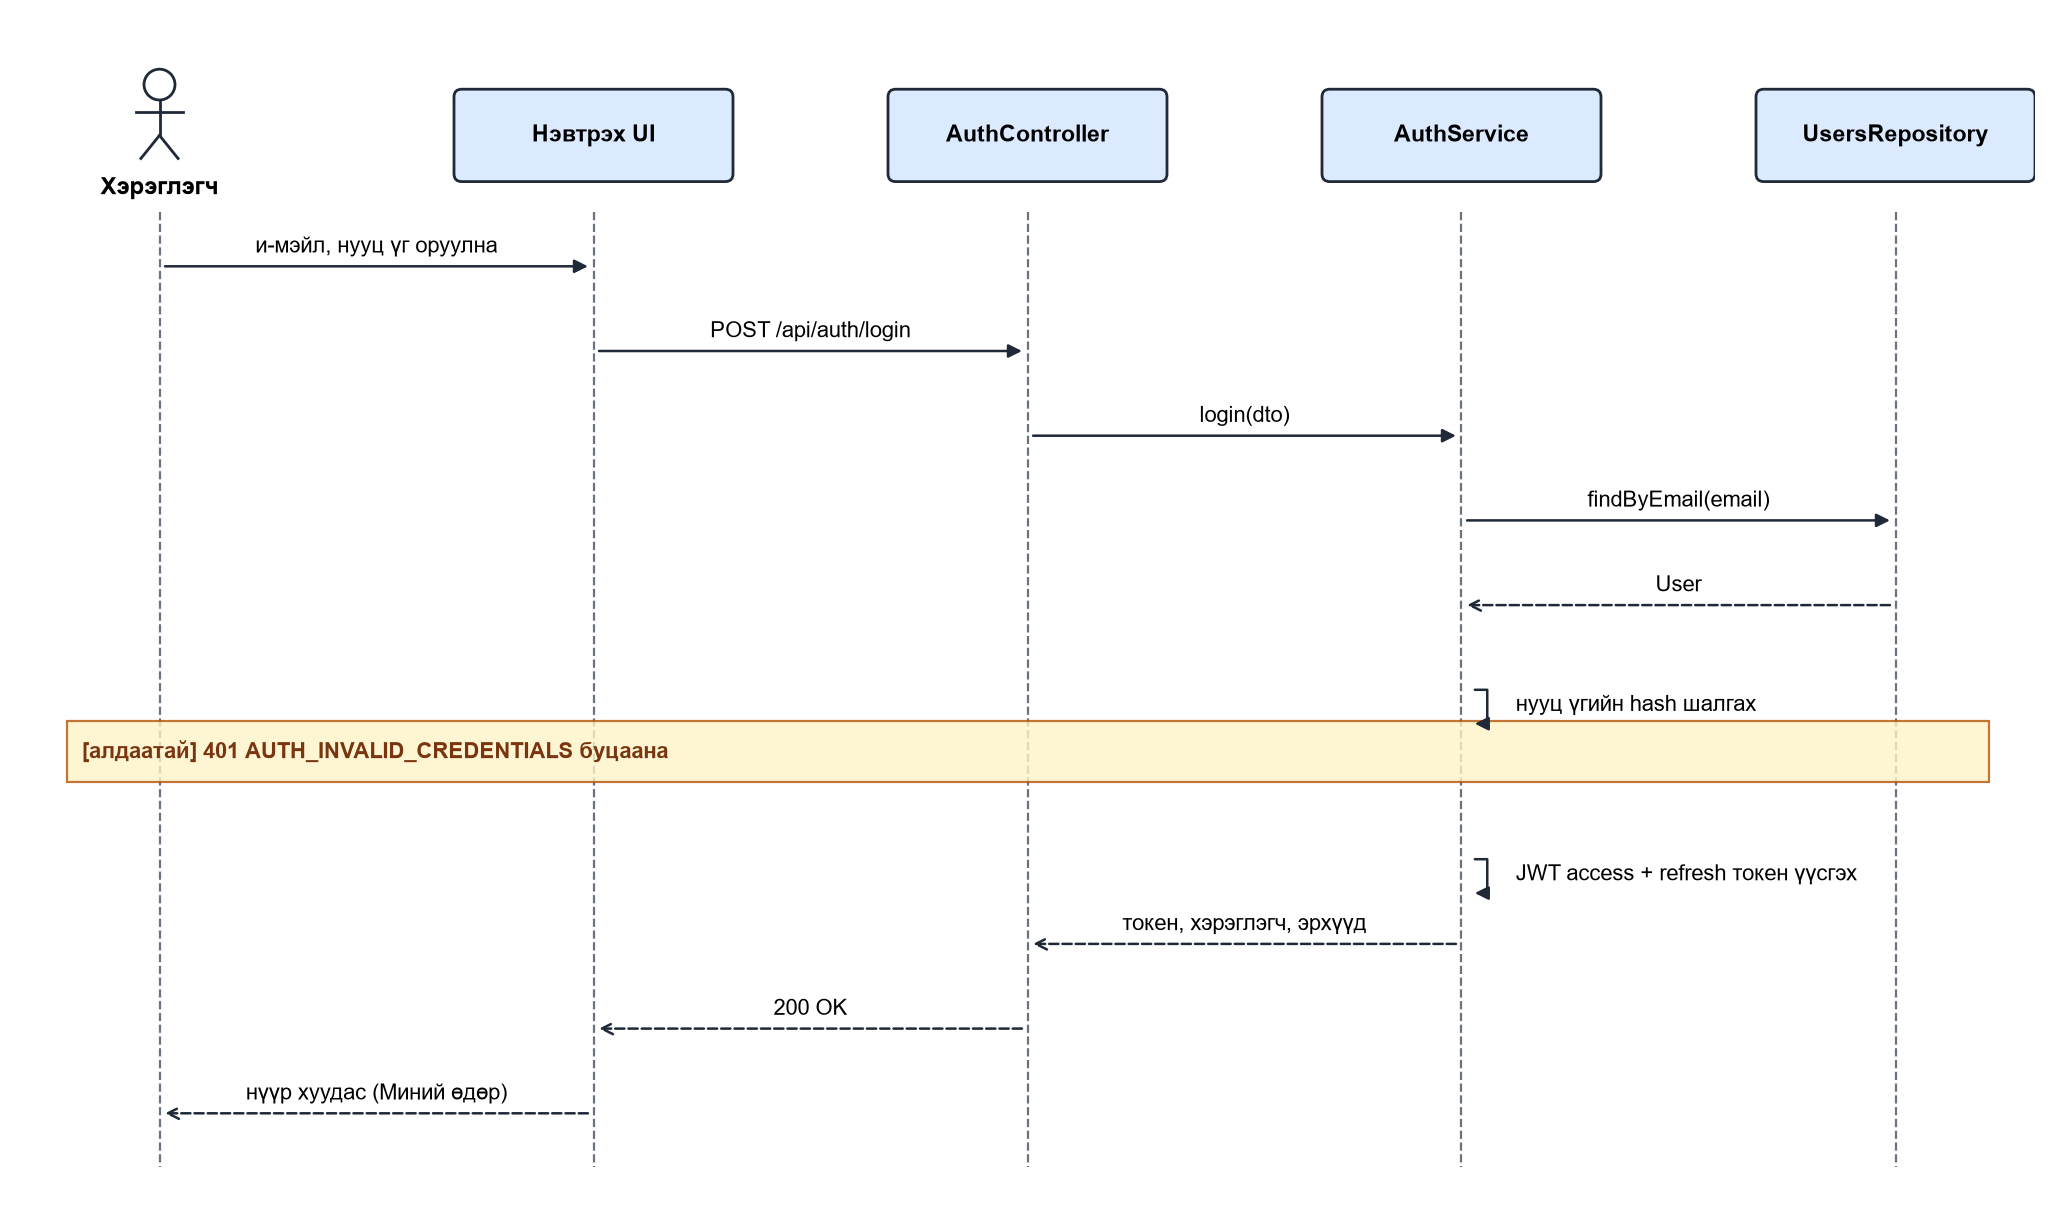
\includegraphics[width=\linewidth]{Figures/seq_login.png}
\caption{Нэвтрэх дарааллын диаграмм}
\label{fig:seqLogin}
\end{figure}

\begin{figure}[H]
\centering
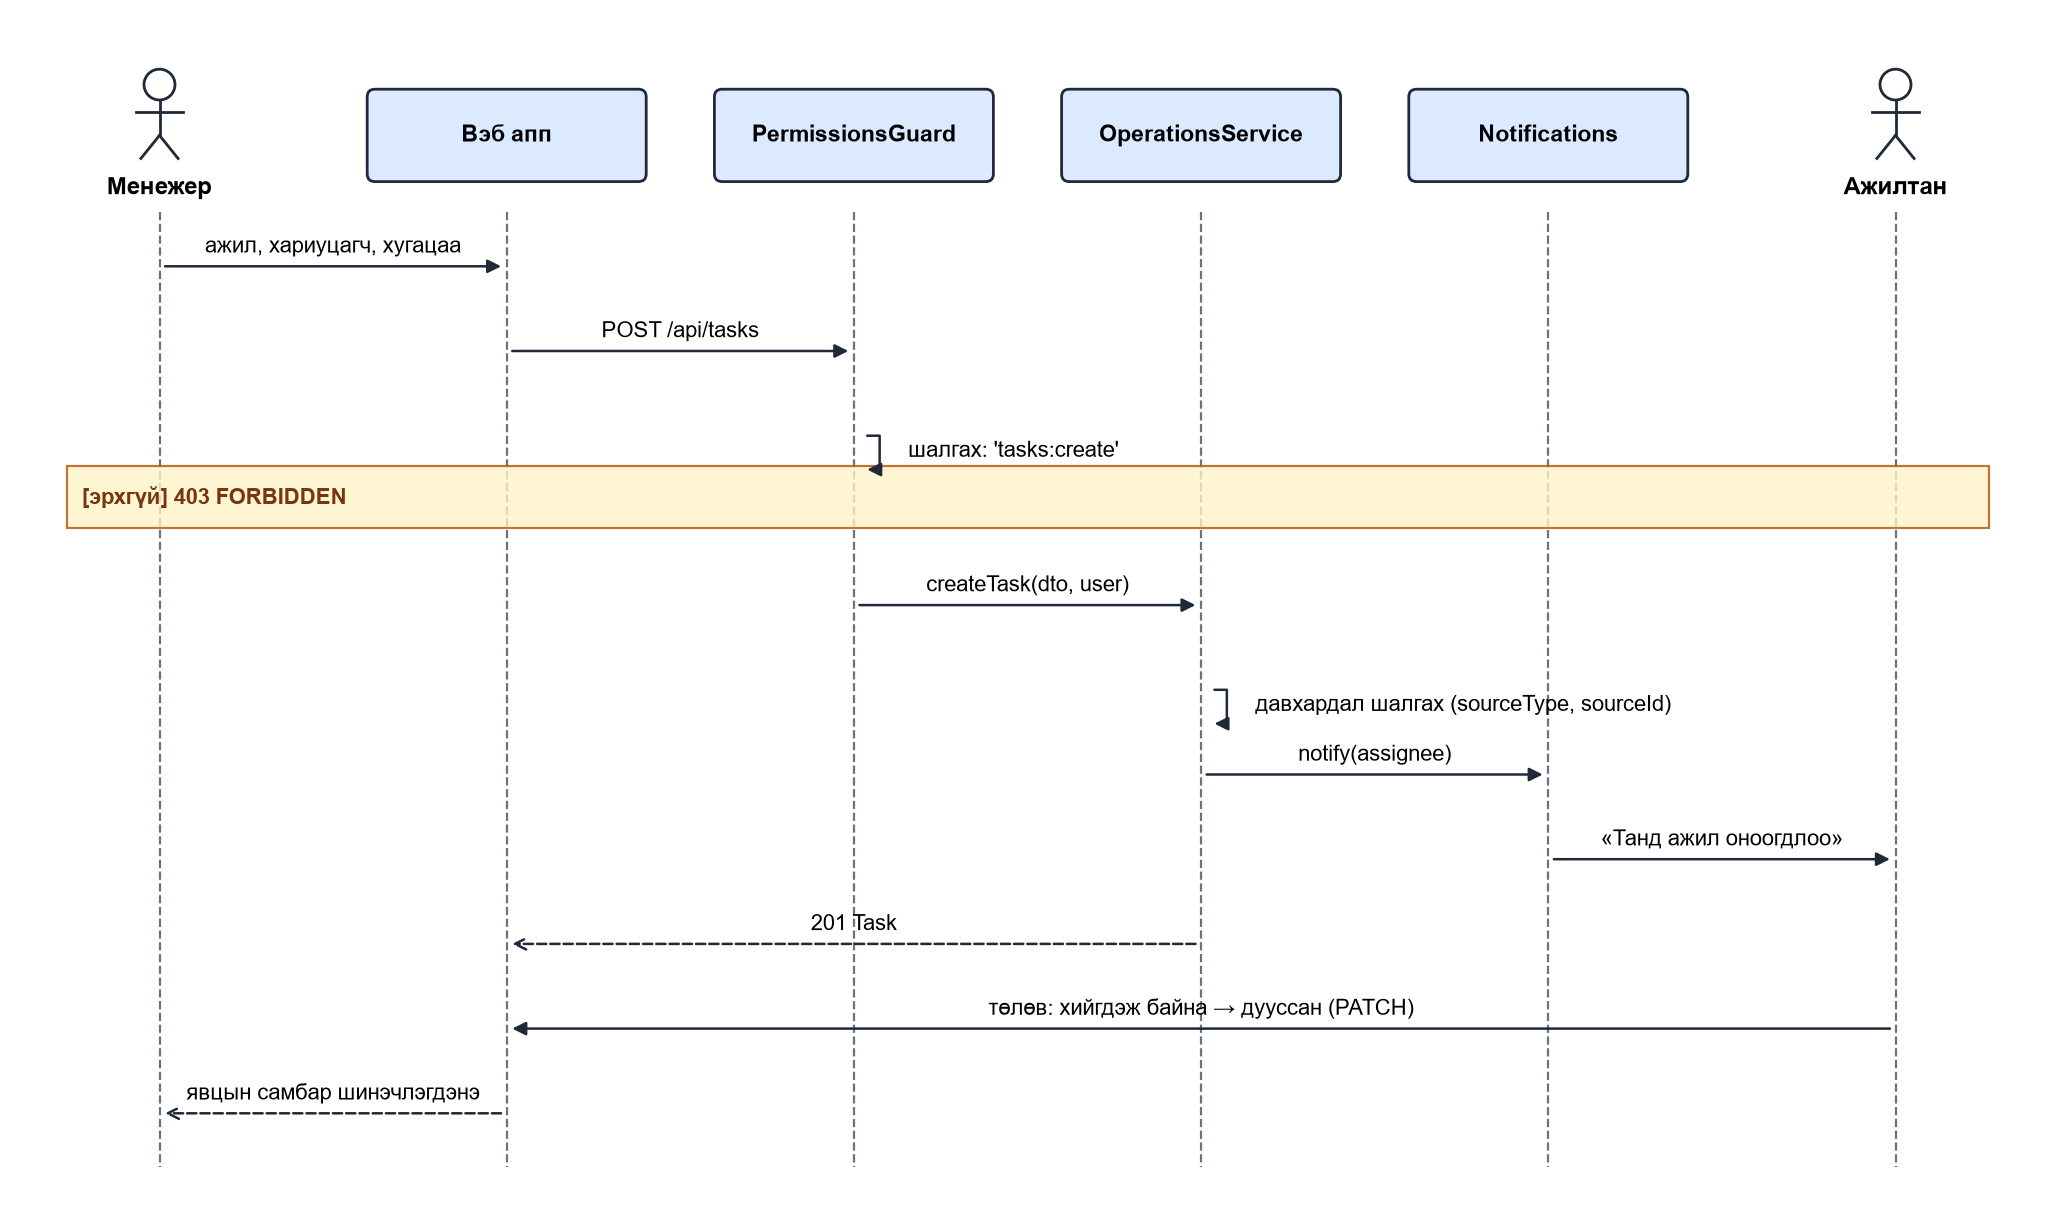
\includegraphics[width=\linewidth]{Figures/seq_task.png}
\caption{Ажил оноох дарааллын диаграмм}
\label{fig:seqTask}
\end{figure}

%-------------------------------------------------------------------------------
\section{Үйл ажиллагааны диаграмм}
Зураг~\ref{fig:activity}-д ажил оноогдохоос дуусах хүртэлх менежер, систем, ажилтны үйл ажиллагааг харуулав.

\begin{figure}[H]
\centering
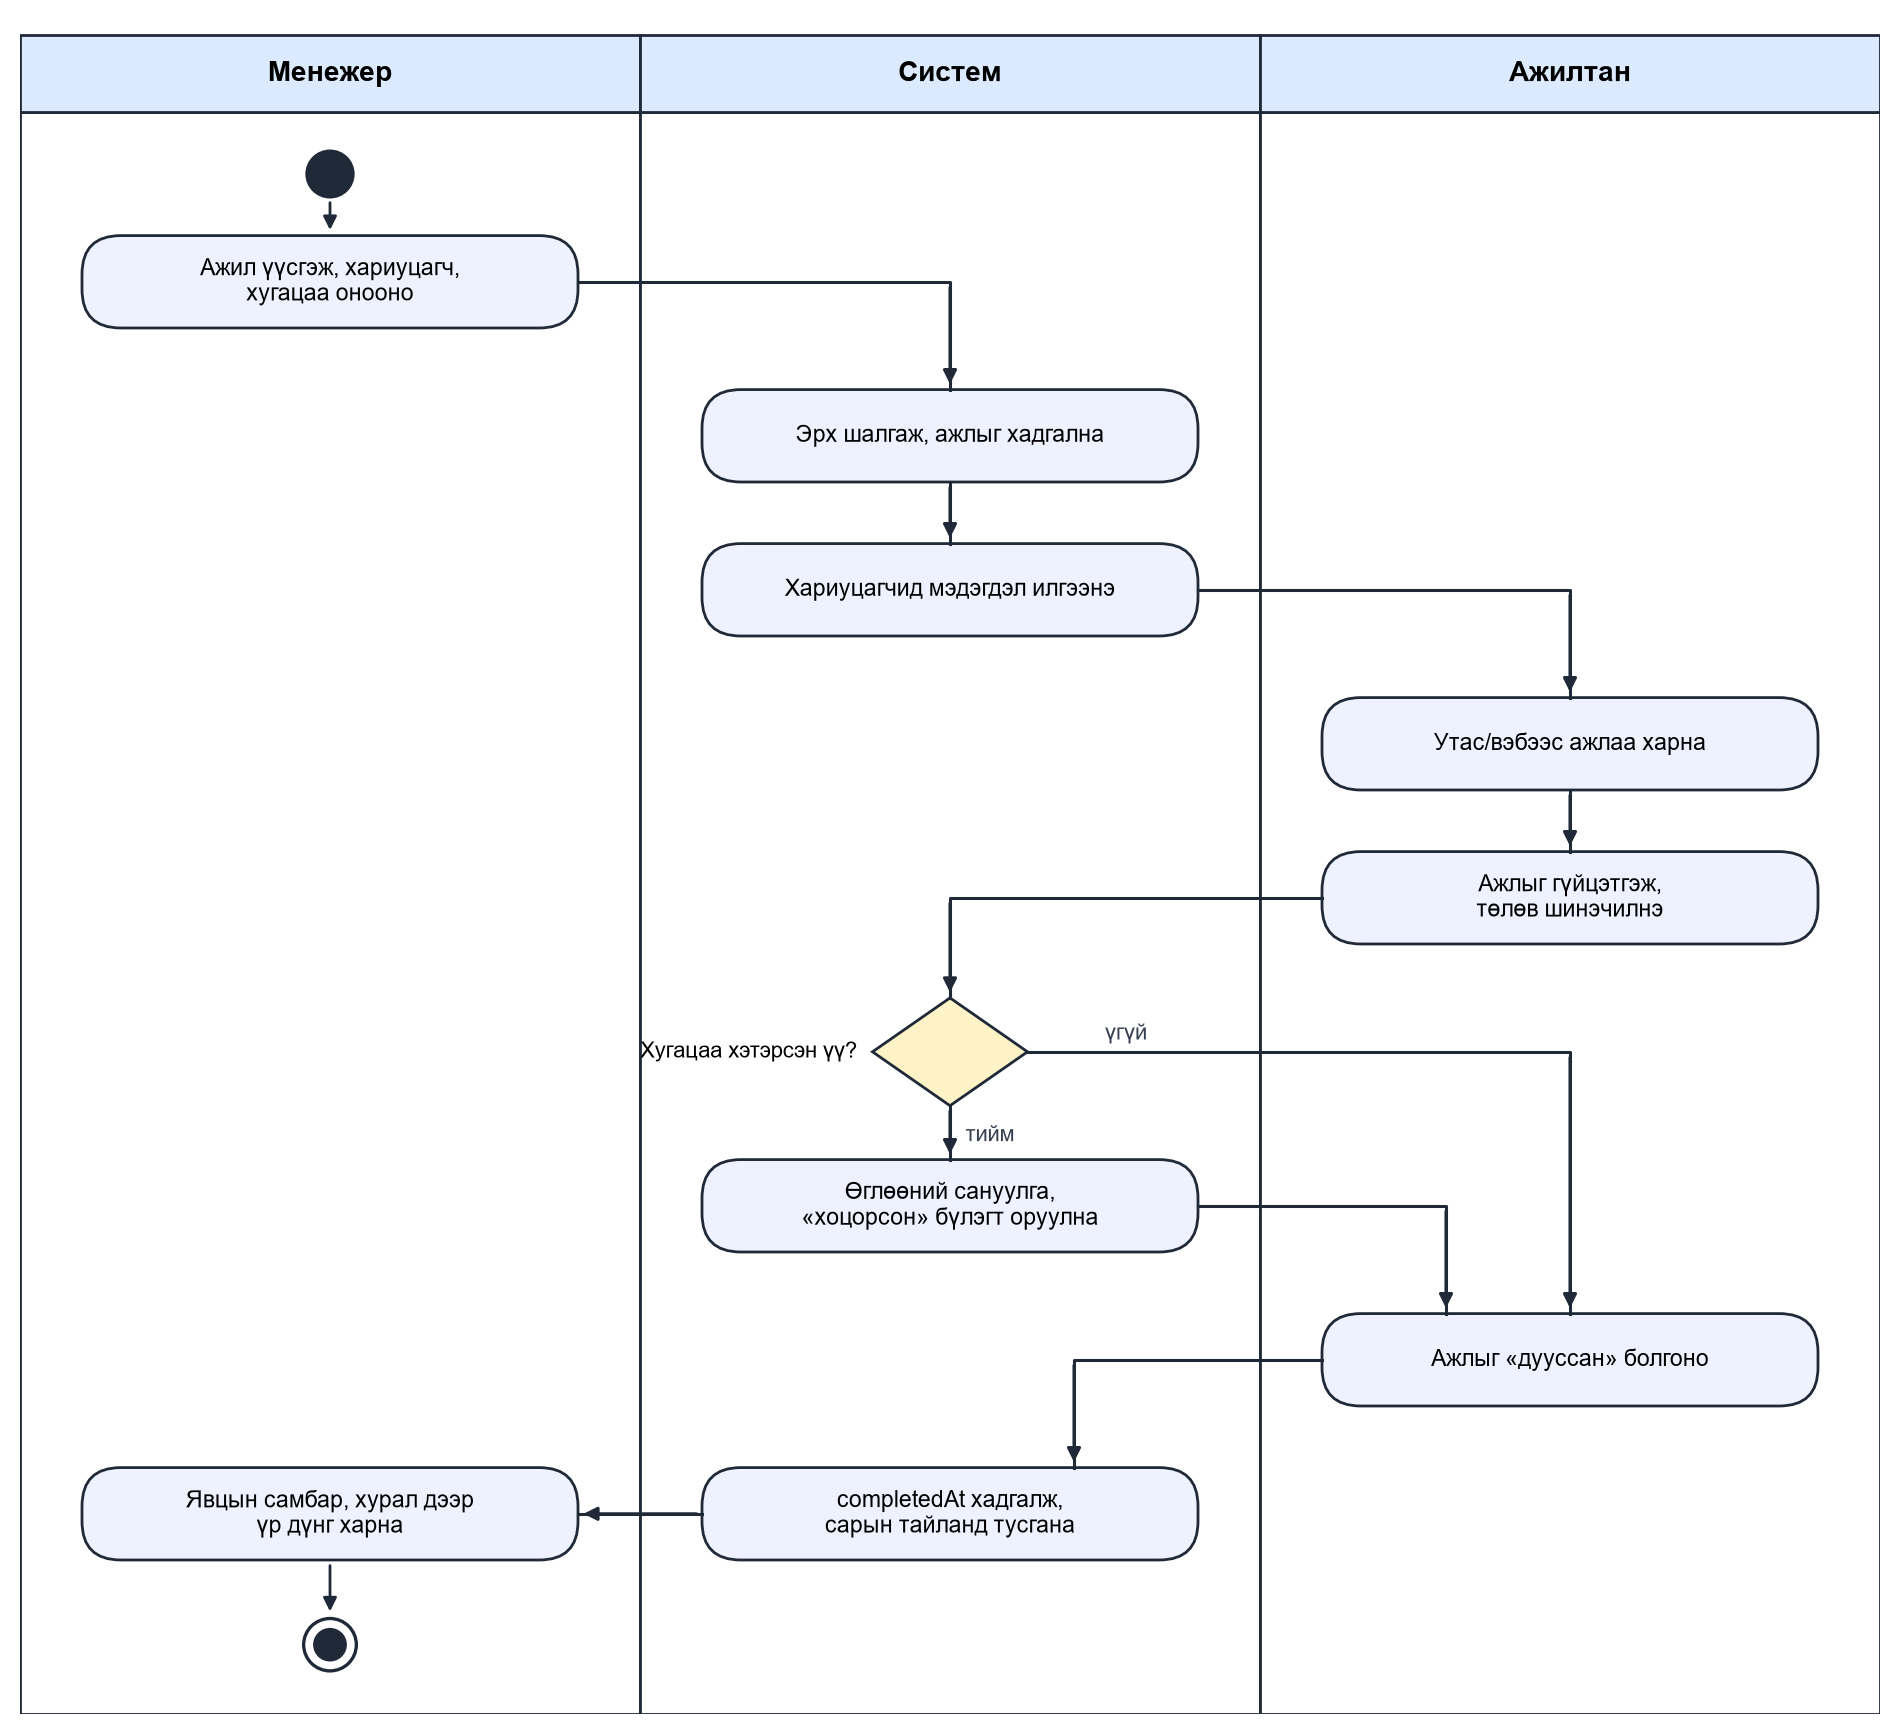
\includegraphics[width=0.9\linewidth]{Figures/activity_task.png}
\caption{Ажлын үйл ажиллагааны диаграмм}
\label{fig:activity}
\end{figure}

\section*{Бүлгийн дүгнэлт}
Энэ бүлэгт системийн үйл ажиллагааг хэрэглэгчийн дүрээр тодорхойлж, 22 функциональ, 10 функциональ бус шаардлага боловсруулав. Use-case диаграмм, есөн use-case-ийн дэлгэрэнгүй тодорхойлолт, шаардлагын мөрдөх матриц, шинжилгээний класс, дараалал, үйл ажиллагааны диаграммаар системийн зан төлөвийг загварчлав.
